%%%%%%%%%%%%%%%%%%%%%%%%%%%%%%%%%%%%%%%%%
% University Assignment Title Page 
% LaTeX Template
%
% This template has been downloaded from:
% http://www.latextemplates.com
%
% Original author:
% WikiBooks (http://en.wikibooks.org/wiki/LaTeX/Title_Creation)
% 
% Instructions for using this template:
% This title page is presently capable of being compiled as is. This is not 
% useful for including it in another document. To do this, you have two options: 
%
% 1) Copy/paste everything between \begin{document} and \end{document} 
% starting at \begin{titlepage} and paste this into another LaTeX file where you 
% want your title page.
% OR
% 2) Remove everything outside the \begin{titlepage} and \end{titlepage} and 
% move this file to the same directory as the LaTeX file you wish to add it to. 
% Then add \input{./title_page_1.tex} to your LaTeX file where you want your
% title page.
%
%%%%%%%%%%%%%%%%%%%%%%%%%%%%%%%%%%%%%%%%%

%----------------------------------------------------------------------------------------
%    PACKAGES AND OTHER DOCUMENT CONFIGURATIONS
%----------------------------------------------------------------------------------------

\documentclass[12pt]{article}
\usepackage[utf8]{inputenc}
\usepackage[T2A]{fontenc}
\usepackage[ukrainian,russian]{babel}
\usepackage[numbers,sort&compress]{natbib}
\usepackage{amsfonts,amsmath,amsxtra,amsthm,amssymb,latexsym}
%\usepackage[left=4cm,right=4cm,
%    top=2cm,bottom=2cm,bindingoffset=0cm]{geometry}

\usepackage{natbib}
\usepackage{graphicx}
\usepackage{listings}

\begin{document}

\begin{titlepage}

\newcommand{\HRule}{\rule{\linewidth}{0.5mm}} % Defines a new command for the horizontal lines, change thickness here

\center % Center everything on the page
 
%----------------------------------------------------------------------------------------
%	HEADING SECTIONS
%----------------------------------------------------------------------------------------

\textsc{\LARGE МОСКОВСКИЙ ГОСУДАРСТВЕННЫЙ УНИВЕРСИТЕТ}\\[0.2cm] % Name of your university/college
\textsc{\LARGE имени М.В. Ломоносова}\\[0.5cm] % Major heading such as course name
\textsc{\Large Факультет вычислительной математики и кибернетики}\\[0.5cm] % Minor heading such as course title
\textsc{\large Кафедра оптимального управления}\\[2.5cm] % Minor heading such as course title

%----------------------------------------------------------------------------------------
%	TITLE SECTION
%----------------------------------------------------------------------------------------

\HRule \\[0.4cm]
{ \huge \bfseries Отчет}\\[0.2cm] % Title of your document
\textsc{о проделанной работе в рамках практикума\\на ЭВМ в 6 семестре}
\HRule \\[1.5cm]
 
%----------------------------------------------------------------------------------------
%	AUTHOR SECTION
%----------------------------------------------------------------------------------------

\begin{minipage}{0.3\textwidth}
\begin{flushleft} 
\emph{Автор:}\\
Павел Кириллович \textsc{Ахрамеев}\\ % Your name
\textsc{}\\
\textsc{}\\
\end{flushleft}
\end{minipage}
~
\begin{minipage}{0.6\textwidth}
\begin{flushright} 
\emph{Руководители:} \\
Борис Александрович \textsc{Будак}\\ % Supervisor's Name
Юрий Николаевич \textsc{Киселев}\\ % Supervisor's Name
Сергей Николаевич \textsc{Аввакумов}\\ % Supervisor's Name
Анастасия Владимировна \textsc{Ничипорчук}\\ % Supervisor's Name
\end{flushright}
\end{minipage}\\[4cm]

% If you don't want a supervisor, uncomment the two lines below and remove the section above
%\Large \emph{Author:}\\
%John \textsc{Smith}\\[3cm] % Your name

%----------------------------------------------------------------------------------------
%	DATE SECTION
%----------------------------------------------------------------------------------------

{\large Москва --- \the\year}\\[1cm] % Date, change the \today to a set date if you want to be precise

%----------------------------------------------------------------------------------------
%	LOGO SECTION
%----------------------------------------------------------------------------------------

%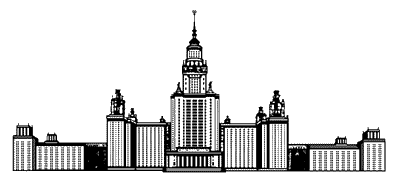
\includegraphics[height=1cm]{msu_logo.png} % Include a department/university logo - this will require the graphicx package
 
%----------------------------------------------------------------------------------------

\vfill % Fill the rest of the page with whitespace

\end{titlepage}
\setcounter{page}{2}
\tableofcontents
\newpage

\section {Постановка задачи}
\tolerance
В рамках практикума на ЭВМ VI семестра 
кафедры оптимального управ\-ления 
факультета ВМК МГУ необходимо было реализовать программу 
для решения краевых задач методом продолжения по параметру. 
Стро\-гая математическая постановка задания будет изложена далее.
\section {Теоретическое описание метода}
\tolerance
Рассматриваем краевую задачу
\begin {equation}
\label {edged_problem}
\begin{cases} 
x\dot = f(t,x), a\leq t\leq b, \\
R(x(a),x(b)) = 0,\\
x\in\mathbb{E}^n.
\end{cases}
\end{equation}

Здесь $f(t,x):\mathbb{E}^1\times\mathbb{E}^n\to\mathbb{E}^n, R(x,y):\mathbb{E}^n\times\mathbb{E}^n\to\mathbb{E}^n$ являются гладкими векторными функциями. Предполагаем, что решение краевой задачи
(\ref{edged_problem}) существует. Выберем точку $t_*\in[a,b]$ и рассмотрим задачу Коши

\begin {equation}
\label {koshi_problem}
\begin{cases} 
x\dot = f(t,x), a\leq t\leq b, \\
x|_{t=t_*}=p\in\mathbb{E}^n.
\end{cases}
\end{equation}

Пусть
\begin{equation}
\label{koshi_solution}
x(t,p),  a\leq t\leq b,
\end{equation}
--- решение задачи Коши (\ref{koshi_problem}). Предполагается продолжимость решения (\ref{koshi_solution}) на весь отрезок $[a; b]$ для любого $p$. Начальное значение параметра $p\in\mathbb{E}^n$ ищется из условий выполнения векторного граничного условия в задаче (\ref{edged_problem}), т.е. искомое $p$ является решением уравнения
\begin{equation}
\label{p_problem}
\Phi(p)\equiv R(x(a,p),x(b,p))=0.
\end{equation}

Итак, краевая задача (\ref{edged_problem}) сведена к конечному векторному
уравнению (\ref{p_problem}). Далее к уравнению (\ref{p_problem}) применяется метод продолжения
по параметру. Для этого рассмотрим вспомогательное уравнение
\begin{equation}
\label{p_mu_problem}
\Phi(p(\mu))=(1-\mu)\Phi(p_0), \mu\in[0,1],
\end{equation}
где $p_0\in\mathbb{E}^n$ --- произвольное фиксированное начальное приближение.

Всюду далее считаем выполненными следующие два предложения.
\newtheorem{proposition}{Предположение}
\renewcommand{\theproposition}{\arabic{proposition}}

\begin{proposition}{(о гладкой ветви)}
Уравнение (\ref{p_mu_problem}) при любом $\mu\in[0,1]$ имеет решение
\begin {equation}
\label{plate_eq}
p=p(\mu), 0\leq\mu\leq1,
\end{equation}
функция (\ref{plate_eq}) является гладкой функцией параметра $\mu$ и удовлетворяет
начальному условию
\begin{equation}
\label{p_mu_start}
p(\mu)|{\mu=0}=p_0.
\end{equation}
\end{proposition}
\begin{proposition}{(о невырожденности)}
Матрица
\begin{equation}
\label{dPhi}
\Phi'(p)=(\partial\Phi_i(p)/\partial p_j)^n_{i,j=1},
\end{equation}
невырождена вдоль $p\mu$
\end{proposition}

Справедливость {\bf Предположений 1, 2} зависит от уравнения (\ref{p_problem}) и
от выбора точки $p_0$. Конечно, прямая проверка {\bf Предположений 1, 2} в
сложных нелинейных задачах невозможна. Успешное завершение вычислительного процесса может служить косвенным подтверждением выполнения этих предположений.

Продифференцируем тождество (\ref{p_mu_problem}) по $\mu$:
\begin{equation}
\label{dPhi_mu}
\Phi'(p(\mu))\frac{dp(\mu)}{d\mu}=-\Phi(p_0).
\end{equation}

Из {\bf Предположения 1} и формулы (\ref{dPhi_mu}) следует, что функция $p(\mu)$ является решением векторной задачи Коши
\begin {equation}
\label{external}
\begin{cases}
\frac{dp}{d\mu}=-[\Phi]^{-1}\Phi(p_0), 0\leq\mu\leq1,\\
p(0)=p_0.
\end{cases}
\end{equation}
Численное решение задачи Коши (\ref{external}) позволяет найти функцию $p(\mu),\\0\leq\mu\leq 1;$ вектор
\begin{equation}
\label{p_mu_1}
p(\mu)|{\mu=1}
\end{equation}
должен быть точным решением (\ref{p_problem}) в идеальной ситуации точного нахождения $p(\mu)$. В реальных вычисления вектор (\ref{p_mu_1}) дает новое приближение для решения; точность решения зависит от использованного численного метода и его параметров. Один шаг итерационной процедуры ассоциируется
с решением задачи Коши (\ref{external}). Итерационный процесс $p^0, p^1, p^2,\dots$ поиска решения уравнения (\ref{p_problem}) представим схемой
\begin{equation}
\label{iterative_process}
p^0\xrightarrow[p_0=p^0]{(\ref{external})}p^1=p(\mu)|_{\mu=1}\xrightarrow[p_0=p^1]{(\ref{external})}p^2=p(\mu)|_{\mu=1}\xrightarrow[p_0=p^2]{(\ref{external})}p^3\dots
\end{equation}

В нашей задаче матрица $\Phi'(p)$ имеет вид
\begin{equation*}
\Phi'(p)=R'_x\frac{\partial x(a,p)}{\partial p}+R'_y\frac{\partial x(b,p)}{\partial p}.
\end{equation*}
Здесь $(n\times n) -$ матрицы $R'_x(x,y), R'_y(x,y)$ вычисляются вдоль решения (\ref{koshi_solution}), т.е. при $x=x(a,p), y=y(b,p).$ Введем обозначение
\begin{equation*}
X(t,p)=\frac{\partial x(t,p)}{\partial p} 
\end{equation*}
для $(n\times n) -$ матрицы производных решения (\ref{koshi_solution}) по начальному условию. Матрица $X(t,p)$ определяется дифференциальным уравнением в вариациях
\begin{equation*}
\begin{cases}
X\dot=AX, a\leq t\leq b,\\
X|_{t=t_0}=I,
\end{cases}
\end{equation*}
где $A=A(t,p)=f'_x(t,x)|_{x=x(t,p)}$ есть $(n\times n) -$ матрица, $I$ --- единичная матрица. Для одновременного вычисления векторной функции $x(t,p)$ и матричной функции $X(t, p)$ может быть записана следующая векторно-матричная задача Коши
\begin{equation}
\label{internal}
\begin{cases}
x\dot=f(t,x), x|_{t=t_*}=p,\\
X\dot=f'_x(t,x)X, X|_{t=t_*}=I, a\leq t\leq b.
\end{cases}
\end{equation}

Задачу Коши (\ref{external}) будем называть {\if внешней задачей}, задачу Коши (\ref{internal}) —
{\if внутренней задачей}. Таким образом, предлагается итерационный процесс (\ref{iterative_process}) для решения рассматриваемой краевой задачи (\ref{edged_problem}) на основе внешней задачи (\ref{external}) и внутренней задачи (\ref{internal}). На одном шаге итерационного процесса выпняется решение внешней задачи (\ref{external}), в ходе решения которой происходит многократное обращение к решению внутренней задачи Коши (\ref{internal}) при различных значениях параметра $p$. При формировании
матриц $f'_x, R'_x, R'_y$ привлекаются возможности среды по выполнению аналитических вычислений.
\newpage
\section{Реализация программы}
\tolerance
В программе реализованы:
\begin{enumerate}
\item Описанный выше алгоритм
\item Пользовательский интерфейс
\begin{enumerate}
\item Основной экран программы
\begin{itemize}
\item Поля ввода данных
\begin{itemize}
\item Поле ввода размерности системы дифференциальных уравнений
\item Поля ввода параметров временной сетки: правый и левый концы; шаг сетки
\item Поле ввода параметра $t_*$ для описанного выше алгоритма
\item Поля выбора численных методов решения внешней и внутренний задачи из списка
\begin{enumerate}
\item Рунге-Кутта-Фельберга 2-3
\item Рунге-Кутта-Фельберга 4-5
\item Адамса
\item Эйлера
\end{enumerate}
\item Поля ввода погрешности рассчетов внутренней и внешней задачи
\item Поле ввода количества итераций (вычисления внешней задачи Коши)
\item После вычисления становится доступно поле ввода функц\-ионала и кнопка для его вычисления
\item По кнопке "Показать/скрыть краевую задачу" можно открыть/скрыть таблицу для ввода краевой задачи
\begin {enumerate}
\item Правая часть системы дифференциальных уравнений $f(t,x)$ в формате $x=(x_1,x_2,\dots,x_n)$.\\ Примечание: формат ввода: x1, x2, \dots, xn
\item Краевые условия в виде функции $R(x,y)$ от переменных $x=(x_1,x_2,\dots,x_n)$ и $y=(y_1,y_2,\dots,y_n)$. \\Примечание: формат ввода x1, x2, \dots, xn, y1, y2, \dots, yn
\item Вектор $p_0$ --- вектор начального приближения в итерационном процессе (\ref{iterative_process})
\item Параметр отображения траектории на графике
\end{enumerate}
\end{itemize}
\item Поля вывода результатов
\begin{itemize}
\item Координатная плоскость для вывода графиков
\item Таблица результатов со значениями решения на временной сетке
\end{itemize}
\item Поля настройки отображения данных на графике (применяются по нажатию на кнопку "Обновить")
\begin{itemize}
\item Списки выбора стиля и цвета линии \\Примечание: списки значений легко редактируются тек\-стовым редактором (внимательно изучите содержимое папки \texttt{/Settings} в каталоге программы)
\item Поля для изменения масштаба графиков
\item Поля для вывода конкретной фазовой траектории на графике
\end{itemize}
\end{itemize}
\end{enumerate}
\item Механизм загрузки и сохранения примеров, результатов
\item Редактор таблиц с возможностью экспорта их в MS Excel (требуется MS Excel for Windows\textregistered)
\item Библиотека примеров из книги \cite{oy}
\item Пункты меню "Помощь"  и "О программе"
\end{enumerate}

\newpage
\section{Примеры}
Сравнение результатов работы программы с результатами, приведенными в книге \cite{oy}.
\subsection {Краевая задача двух тел}
\begin{equation*}
\begin{cases}
x_1\dot=x_3,\\
x_2\dot=x_4,\\
x_3\dot=-x_1(x_1^2+x_2^2)^{-3/2},\\
x_4\dot=-x_2(x_1^2+x_2^2)^{-3/2},\\
x_1(0)=2,\\
x_2(0)=0,\\
x_1(7)=1:0738644361,\\
x_2(7)=1:0995343576,\\
t_*=0,\\
p_0^1=[2,0,-0.5,0.5],\\
p_0^2=[2,0,0.5,-0,5].
\end{cases}
\end{equation*}

Библиотека примеров: \texttt{/Examples/edged2figures.mat}.
\newline\\
{\bf Результаты эксперимента}
\begin{itemize}
\item Для вектора $p_0^1$: $p_0=[2, 0, 0, 0.5]$.
\item Для вектора $p_0^2$: $p_0=[2, 0, 0.4511, 0.2994]$
\end{itemize}

Замечу, что результаты эксперимента близки к результатам, указанным в \cite{oy}:
\begin{itemize}
\item $ans1=[2.,0.,0.0000004834,0.5000000745]$, 
\item $ans2=[2.,0.,0.4510782034,-0.2994186665]$.
\end{itemize}

\begin{figure}[h!]
\begin{center}$
\begin{array}{cc}
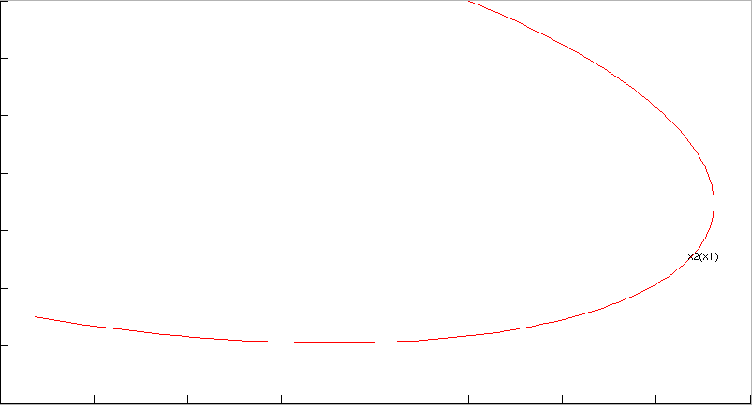
\includegraphics[width=2.5in]{Example1a_12.png} &
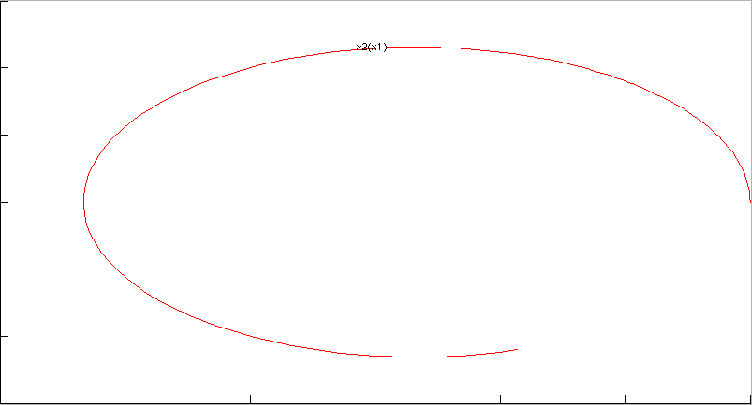
\includegraphics[width=2.5in]{Example1b_12.png}
\end{array}$
\end{center}
\caption{Фазовые траектории $x_2(x_1)$ в обоих случаях}
\label{Example1_pics}
\end{figure}

На рисунке (\ref{Example1_pics}) приведены фазовые траектории $x_2(x_1)$ для \\$p_0^1=[2,0,-0.5,0.5]$ и $p_0^2=[2,0,0.5,-0,5].$
\newpage
\subsection{Предельные циклы в системе Эквейлера}
\begin{equation*}
\begin{cases}
x_1\dot=x_2 x_3,\\
x_2\dot=x_3(-x_1+sin(x_2)),\\
x_3\dot=0,\\
x_4\dot=0,\\
x_1(0)=x_4(0),\\
x_2(0)=0,\\
x_1(1)=x_4(1),\\
x_2(1)=0,\\
t_*=0,\\
p_0^1 = [2, 0, 2\pi, 2],\\
p_0^2 = [6.5, 0, 2\pi, 6.5],\\
p_0^3 = [9, 0, 2\pi, 9],
\end{cases}
\end{equation*}

Библиотека примеров: \texttt{/Examples/limitLoopsInEkveiler.mat}.
\newline\\
{\bf Результаты эксперимента}
\begin{itemize}
\item Для вектора $p_0^1$: $p_0=[3.96554684478714,    -2.62629602035752e-15, \\   6.46614183079246,	3.96554684478714]$.
\item Для вектора $p_0^2$: $p_0=[7.10786344954066,    -2.27592750257336e-18, \\	 6.33878906325561,	7.10786344954066]$
\item Для вектора $p_0^3$: $p_0=[10.2456945992873,    -8.69444146067045e-14, \\ 	6.31011276249781,	10.2456945992873]$
\end{itemize}


Результаты эксперимента, указанные в \cite{oy}:
\begin{itemize}
\item $ans1=[3.9655467678, 0, 6.4661401325,3.9655467678]$, 
\item $ans2=[7.1078664573, 0, 6.3387892836,7.1078664573]$,
\item $ans3=[10.2456910360, 0, 6.3101121791, 10.2456910360]$.
\end{itemize}

\begin{figure}[h!]
\begin{center}$
\begin{array}{cc}
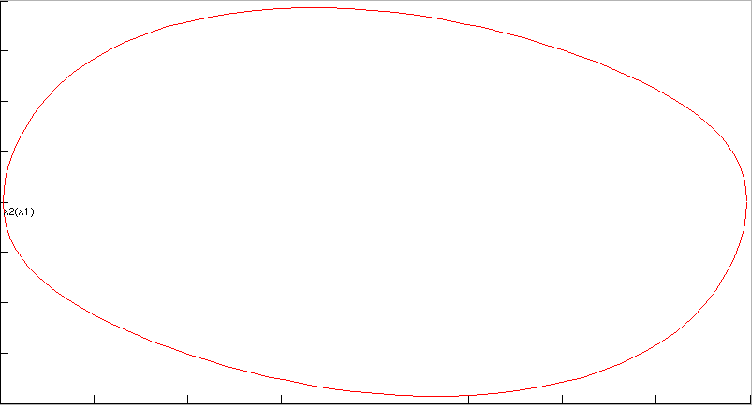
\includegraphics[width=1.7in]{Example2a_12.png} 
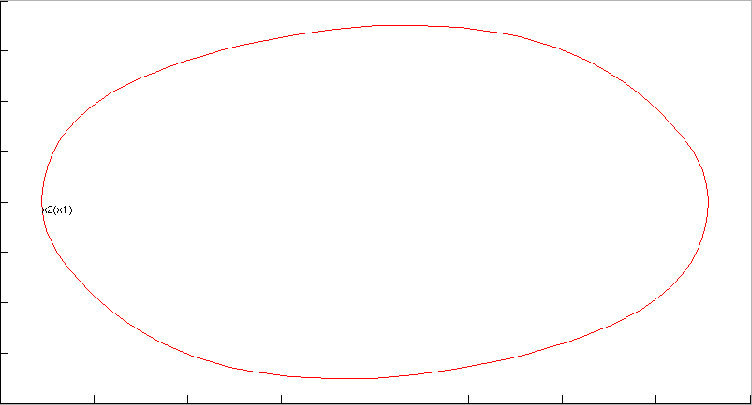
\includegraphics[width=1.7in]{Example2b_12.png} 
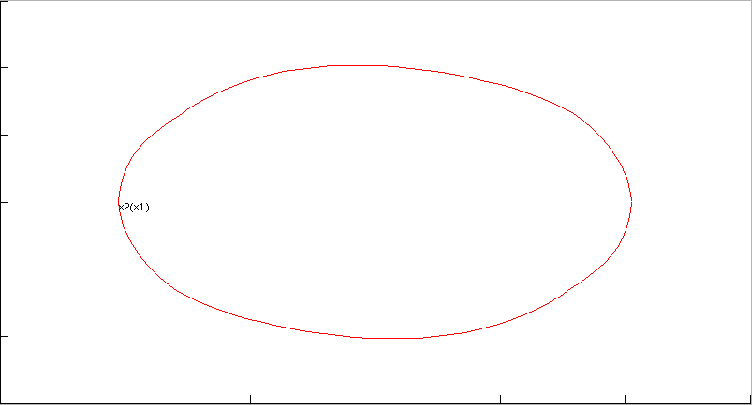
\includegraphics[width=1.7in]{Example2c_12.png}
\end{array}$
\end{center}
\caption{Фазовые траектории $x_2(x_1)$ для $p_0^1, p_0^2$ и $p_0^3$}
\label{Example2_pics}
\end{figure}

На рисунке (\ref{Example2_pics}) приведены фазовые траектории $x_2(x_1)$ для \\$p_0^1 = [2, 0, 2\pi, 2], p_0^2 = [6.5, 0, 2\pi, 6.5]$ и $p_0^3 = [9, 0, 2\pi, 9].$

\subsection{функционал типа “энергия” для трехкратного интегратора}
\begin{equation*}
\begin{cases}
x_1\dot=x_2,\\
x_2\dot=x_3,\\
x_3\dot=\frac{1}{2}(\sqrt{\nu+(x_6+1)^2}-\sqrt{\nu+(x_6-1)^2}),\\
x_4\dot=0,\\
x_5\dot=-x_4,\\
x_6\dot=-x_5,\\
x_1(0)=1,\\
x_2(0)=0,\\
x_3(0)=0,\\
x_1(3.275)=0,\\
x_2(3.275)=0,\\
x_3(3.275)=0,\\
t_*=3.275,\\
p_0 = [0,0,0,-3, 5, -3],\\
\nu=10^{-10}
\end{cases}
\end{equation*}

Библиотека примеров: \texttt{/Examples/energy3integrate.mat}.
\newline\\
{\bf Результат эксперимента}
\newline\\
$p_0=[1.56258154391785e-33,    1.05187183714427e-17,\\	-2.80659384611396e-18,	-2.98505141670188,	4.88802217076114,	-2.90839776271499]$.

Результат, указанный в \cite{oy}:\\
$ans=[0, 0, 0, -2.9850435834, 4.8880088678, -2.9083874537]$.

\begin{figure}[t] 
\begin{center}
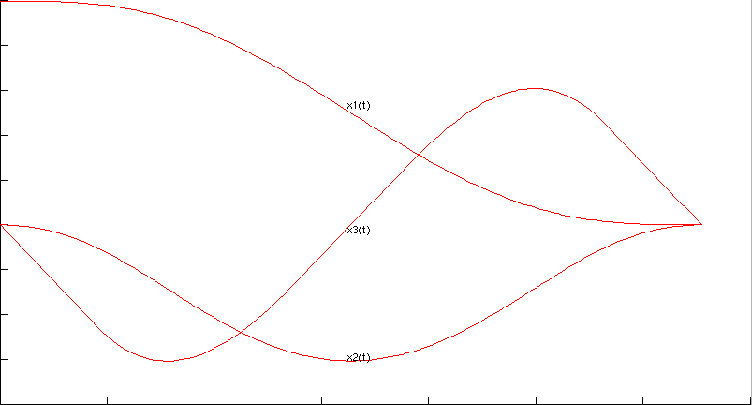
\includegraphics[width=4in]{Example3.png}
\end{center}
\caption{Траектории $x_1(t)$ $x_2(t)$ и $x_3(t)$}
\label{Example3_pic}
\end{figure}
\newpage
\section{Пользовательский интерфейс программы}

\begin{figure}[h!] 
\begin{center}
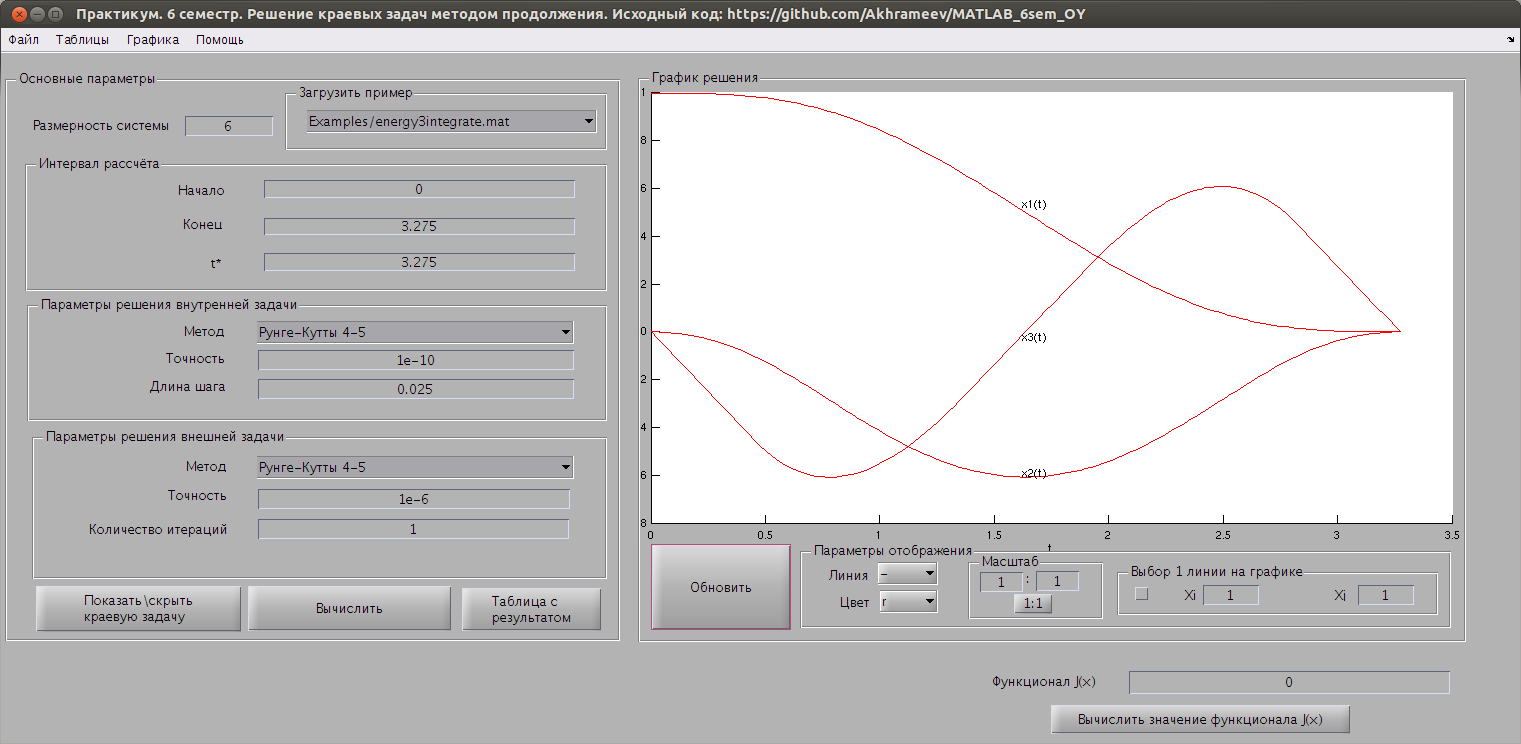
\includegraphics[scale=0.25]{mainWindow.jpeg}
\end{center}
\caption{Главный экран программы после выполнения вычислений}
\label{mainWindow_pic}
\end{figure}

\begin{figure}[h!] 
\begin{center}
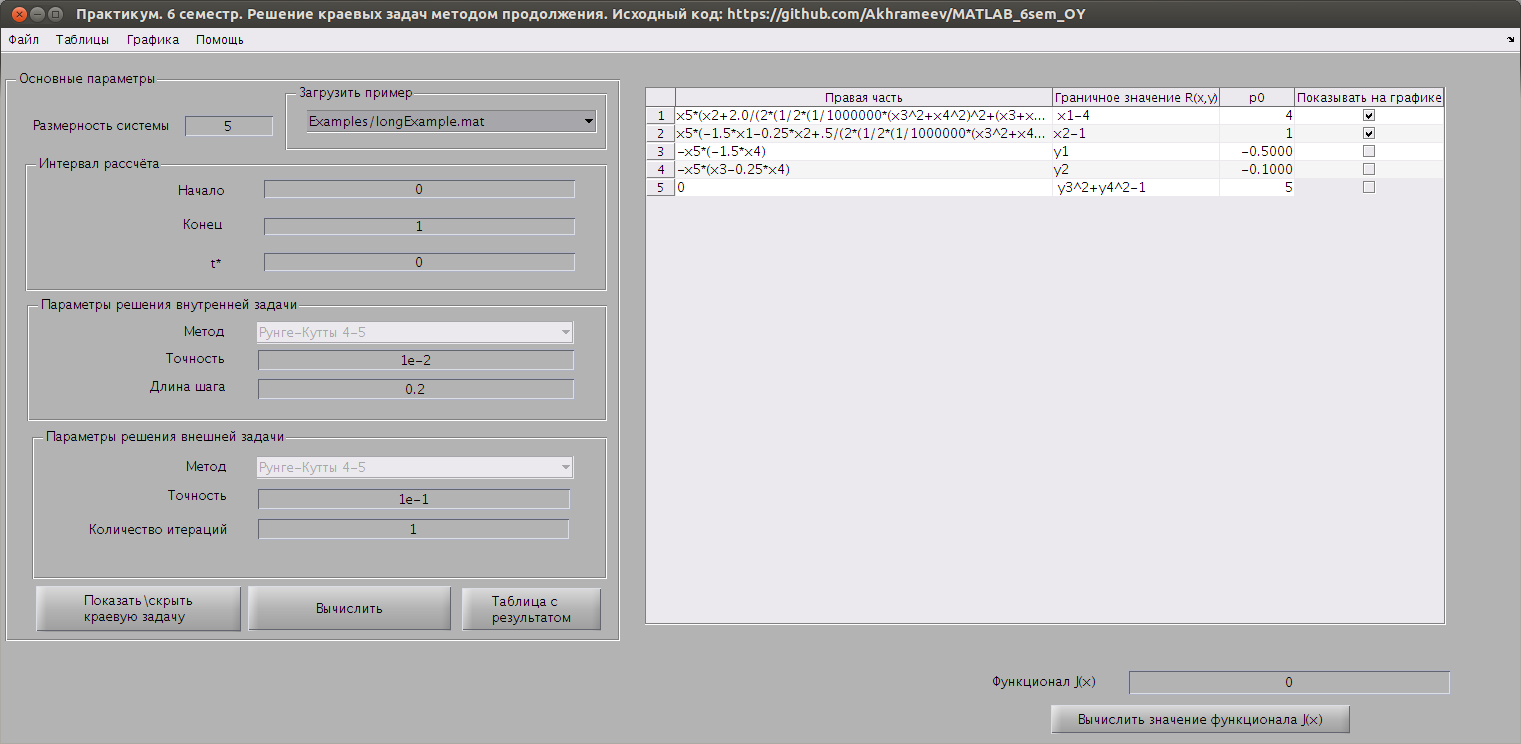
\includegraphics[scale=0.25]{mainWindow_EP.jpeg}
\end{center}
\caption{Главный экран программы: таблица с краевой задачей}
\label{mainWindowPE_pic}
\end{figure}

\begin{figure}[h!] 
\begin{center}
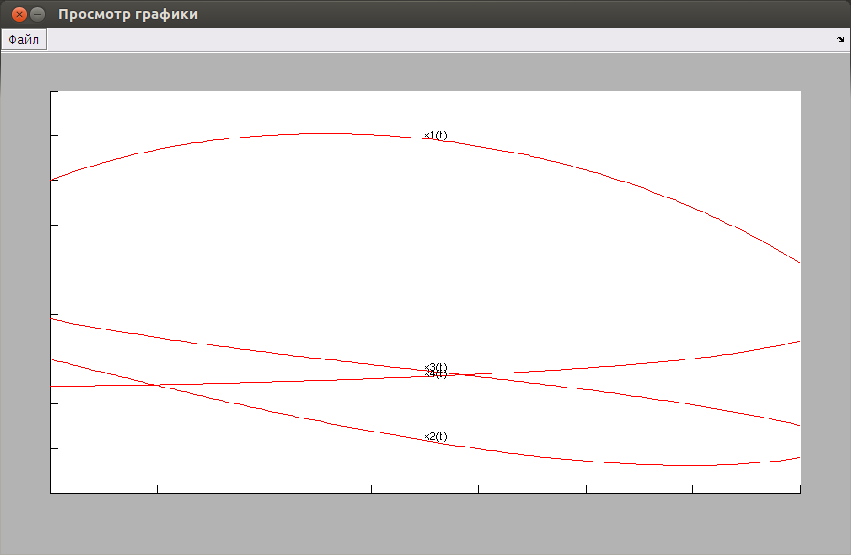
\includegraphics[scale=0.4]{picturesViewer.jpeg}
\end{center}
\caption{Окно просмотра и сохранения изображений}
\label{picViewer_pic}
\end{figure}

\begin{figure}[h!] 
\begin{center}
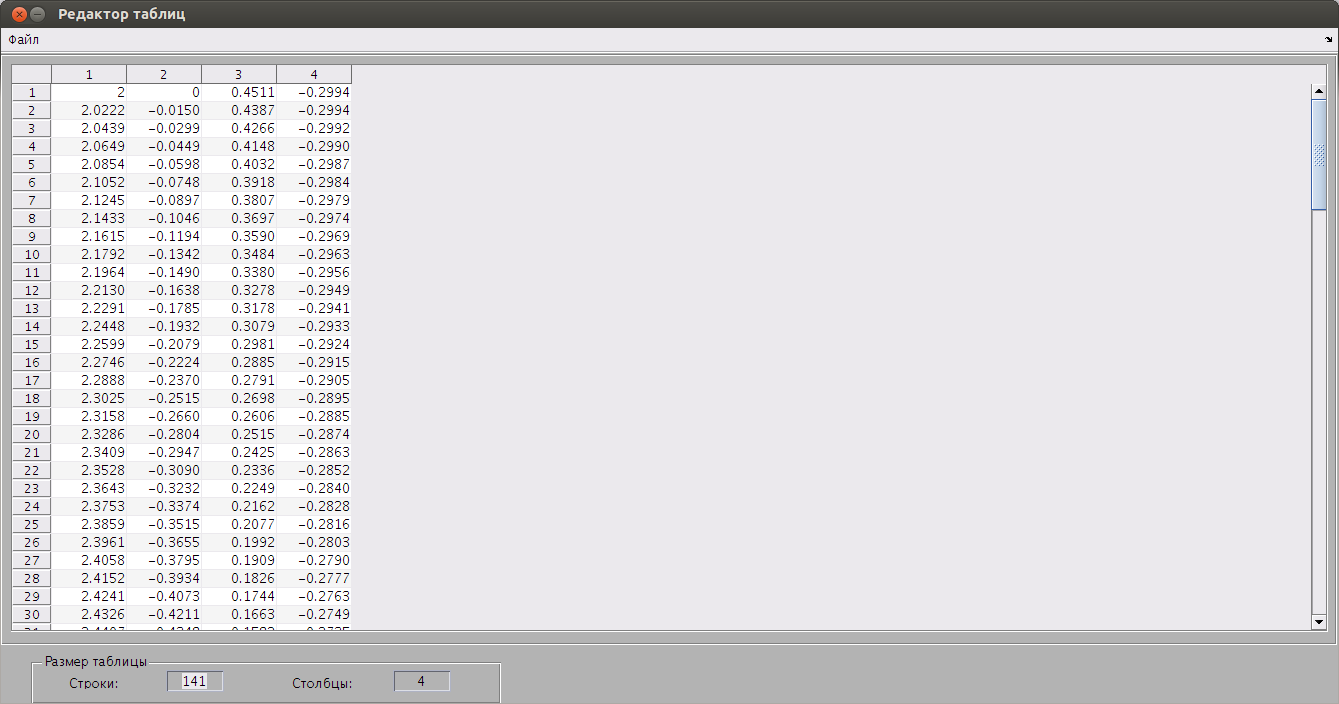
\includegraphics[scale=0.3]{tableEditor.jpeg}
\end{center}
\caption{Редактор таблиц с открытими результатами вычислений}
\label{tableEditor_pic}
\end{figure}

\begin{figure}[h!] 
\begin{center}
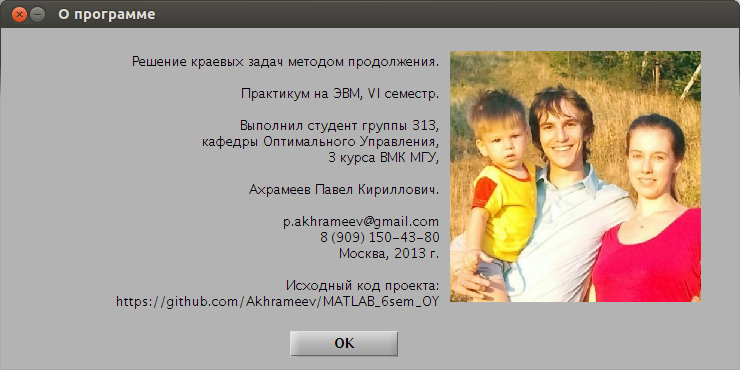
\includegraphics[scale=0.5]{aboutWindow.jpeg}
\end{center}
\caption{О программе}
\label{aboutWindow_pic}
\end{figure}

\begin{figure}[h!] 
\begin{center}
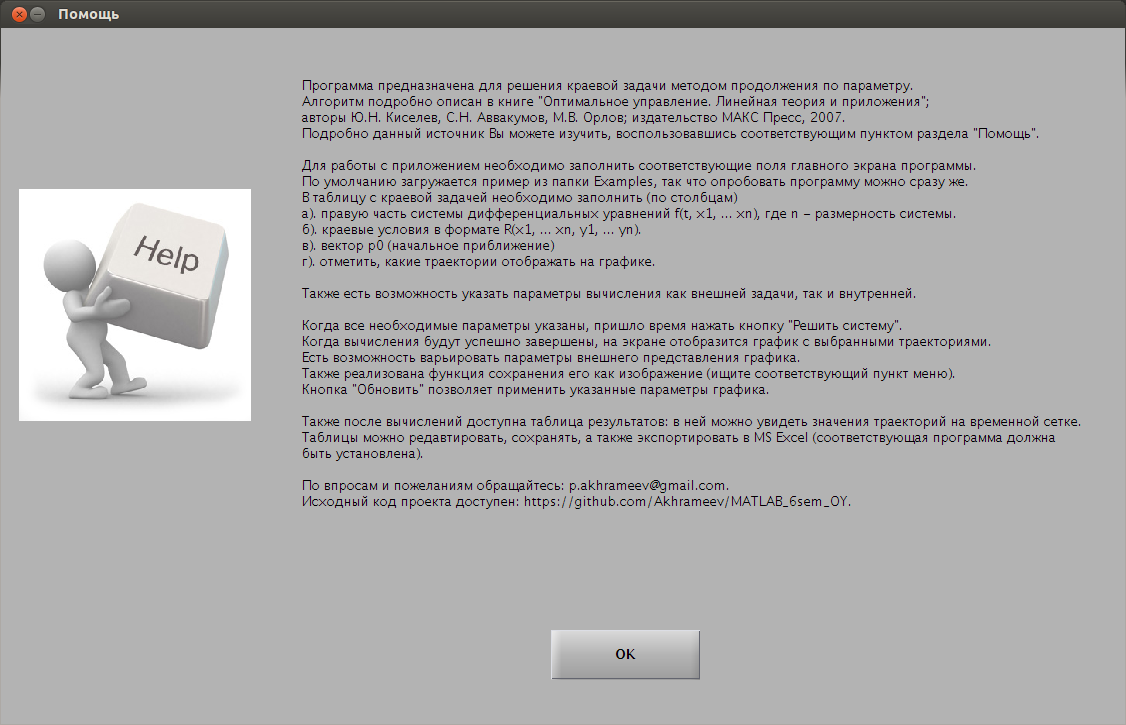
\includegraphics[scale=0.3]{helpWindow.jpeg}
\end{center}
\caption{Помощь}
\label{helpWindow_pic}
\end{figure}
\newpage
\clearpage
\cleardoublepage
\section{Исходный код программы}

Исходный код программы доступен: 
\begin{lstlisting}
https://github.com/Akhrameev/MATLAB_6sem_OY.
\end{lstlisting}
\subsection{Решение внутренней задачи Коши}
\lstset{language=Matlab}   
\begin{lstlisting}
function [ya, yb, Xa, Xb] = solveInternal (p)
global solvingInternalEpsilon; 
global solvingInternalMethod solvingTimeBegin;
global solvingTimeEnd solvingStep;
global systemForSolvingDimension solvingTimeStarred;
n = systemForSolvingDimension;
l = solvingTimeBegin;
r = solvingTimeEnd;
s = solvingStep;
t_s = solvingTimeStarred;
opts = odeset('RelTol', solvingInternalEpsilon);
nMult = n * (n +  1);
q = zeros(1, nMult);
q (1 : n) = p;
I = eye (n);
for i = 1 : n
   q (i * n + 1 : n * (i + 1)) = I (i, :); 
end
if t_s == l
        [~, X] = solvingInternalMethod(@Internal,[l:s:r],q,opts);
elseif t_s == r
        [~, X1] = solvingInternalMethod(@Internal,[r:-s:l],q,opts);
        X = ones (length (X1),nMult);
        X (1 : end, :) = X1 (end:-1:1,:);
else
        [~,X1] = solvingInternalMethod(@Internal,[t_s:-s:l],q,opts);
        [~,X2] = solvingInternalMethod(@Internal,[t_s: s:r],q,opts);
        X = ones(length(X1) + length(X2) - 1, nMult);
        X(1 : length(X1),       :) = X1(end:-1:1, :);
        X(length(X1) + 1 : end, :) = X2(2:end,    :);
end
Xa = zeros (n,n); 
Xb = zeros (n,n);
ya = X(1,   1:n); 
yb = X(end, 1:n);
ya = ya'; 
yb = yb';
for i = 1 : n
    Xa(:,i) = X(1,   i * n + 1 : (i + 1) * n);
    Xb(:,i) = X(end, i * n + 1 : (i + 1) * n);
end
end
\end{lstlisting}

\subsection{Функция создания индикатора выполнения процесса}
\lstset{language=Matlab}  
\begin{lstlisting}
function createWaitbar (handles)
global jProgressbar progressbarOK jInternalProgressbar;
global solvingIterationCount solvingIterationCurrent;
if (progressbarOK)
    
else
    try
        externalProgressbar = handles.externalProgressbar;
        internalProgressbar = handles.internalProgressbar;
        jProgressbarPosition = get (externalProgressbar, 'Position');
        jInternalProgressbarPosition = get (internalProgressbar,...
            'Position');
        jProgressbar = jcontrol(handles.figure1, ...
            javax.swing.JProgressBar(),...
            'Position', jProgressbarPosition, 'Visible', 'off'); 
        jProgressbar.setMaximum (solvingIterationCount);
        jProgressbar.setMinimum (0);
        jProgressbar.setValue (solvingIterationCurrent);
        jProgressbar.setBorderPainted (true);
        jProgressbar.setStringPainted (true);
        jInternalProgressbar = jcontrol (handles.figure1, ...
            javax.swing.JProgressBar(), ...
            'Position', jInternalProgressbarPosition,'Visible','off');        
        jInternalProgressbar.setIndeterminate (true);
        progressbarOK = 1;
    catch
        jProgressbar = 0;
        jInternalProgressbar = 0;
        progressbarOK = 0;
    end;
end
\end{lstlisting}

\subsection{Решение внешней задачи Коши}
\lstset{language=Matlab}  
\begin{lstlisting}
function [ dp ] = solveExternal( count, p )
global q0 ;
updateWaitbar ();
[xa, xb, Xa, Xb] = solveInternal (q0);
F = R(xa, xb);
[xa, xb, Xa, Xb] = solveInternal (p);
dp = -(Rx (xa, xb) * Xa + Ry (xa, xb) * Xb) \ F;
end
\end{lstlisting}

\subsection{Внешняя задача Коши}
\lstset{language=Matlab}  
\begin{lstlisting}
function [ p ] = external (p0, iterationCount)
global solvingExternalEpsilon solvingExternalMethod;
global q0 solvingIterationCurrent;
global pause;
q0 = p0;
opts = odeset('RelTol',solvingExternalEpsilon);
[xa, xb, ~, ~] = solveInternal (p0);
while (solvingIterationCurrent < iterationCount)  
    if (pause)
        break;
    end
    [~, ps] = solvingExternalMethod (@solveExternal, [0 1], p0, opts);
    if norm(R (xa, xb)) >= solvingExternalEpsilon   
        q0 = ps (end, :);
    end
    [xa, xb, ~, ~] = solveInternal (q0);
    solvingIterationCurrent = solvingIterationCurrent + 1;
end
p = q0;
end
\end{lstlisting}

\subsection{Функция сохранения графиков}
\lstset{language=Matlab}  
\begin{lstlisting}
function SaveMenuItem_Callback(hObject, eventdata, handles)
% hObject    handle to SaveMenuItem (see GCBO)
% eventdata  reserved - to be defined in a future version of MATLAB
% handles    structure with handles and user data (see GUIDATA)
tableList = getAllFiles ('Graphics/');
listSize = size(tableList);
listSize = listSize(2);
defaultName = strcat ('Graphics/graphic', num2str(listSize + 1), '.png');
filename = uiputfile ('Graphics/', 'Save current graphic', defaultName);
if (filename == 0)
    return;
end
filename = strcat ('Graphics/', filename);
F = getframe(handles.axes1);
image(F.cdata);
axis ('image');
axis ('off');
try
    imwrite(F.cdata, filename);
catch
    filename = strcat (filename, '.png');
    imwrite (F.cdata, filename);
end
\end{lstlisting}
\newpage
\bibliographystyle{named}
\bibliography{references}
\end{document}